% Standalone native TikZ source. Compile in a temporary output directory:
% pdflatex -halt-on-error -output-directory=<temporary-directory> directed-tree-volume.tex
% The SVG and PNG are direct page exports of the resulting PDF.
\documentclass[tikz,border=12pt]{standalone}
\usepackage[T1]{fontenc}
\usepackage{lmodern,amsmath}
\definecolor{ink}{HTML}{183444}
\definecolor{blue}{HTML}{1B6780}
\definecolor{amber}{HTML}{AD601A}
\begin{document}
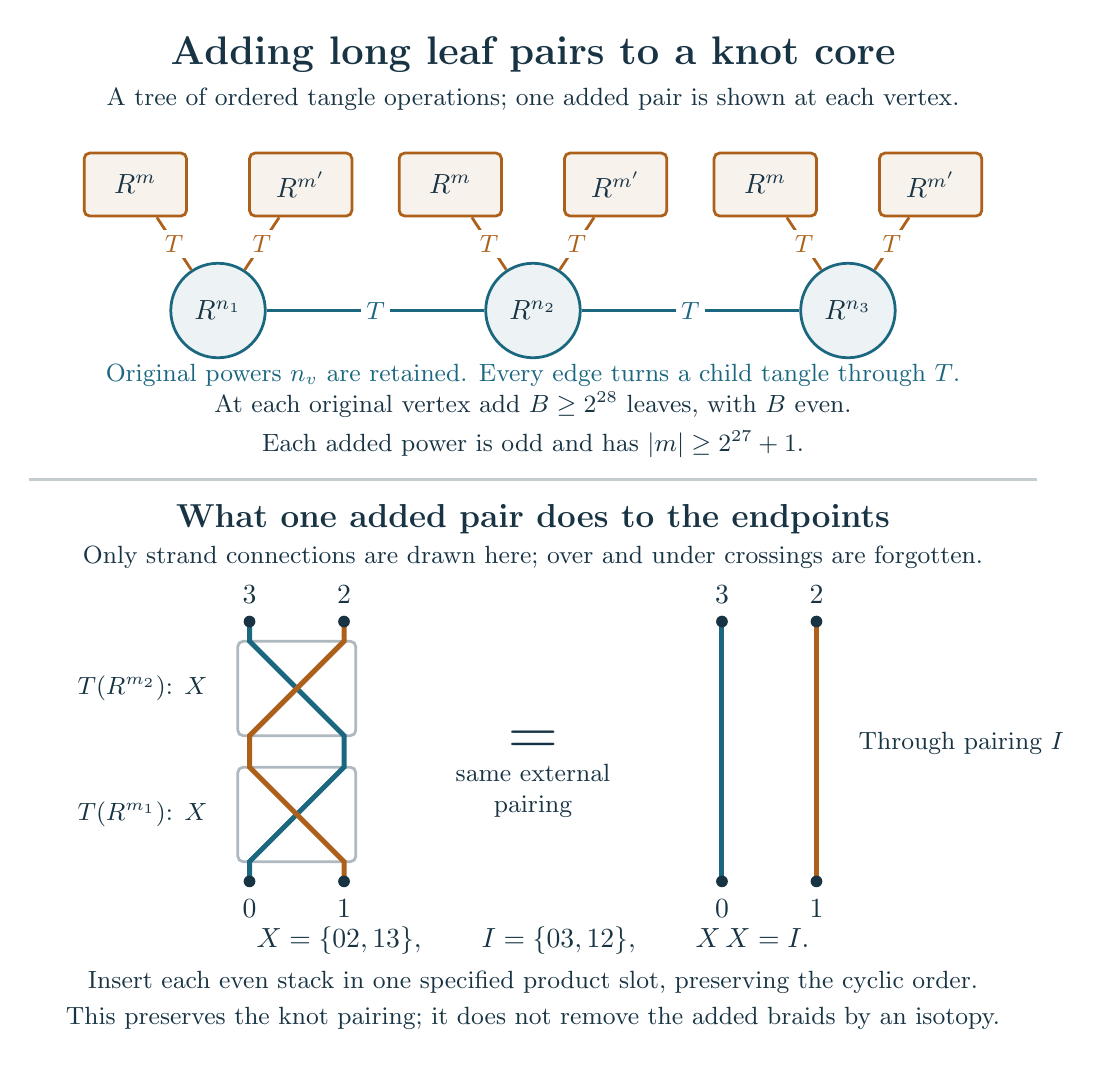
\begin{tikzpicture}[
  font=\sffamily,text=ink,line width=1pt,
  core/.style={circle,draw=blue,fill=blue!8,minimum size=12mm,inner sep=0pt},
  leaf/.style={rounded corners=2pt,draw=amber,fill=amber!8,
    minimum width=13mm,minimum height=8mm},
  turn/.style={fill=white,inner sep=2pt,font=\small},
  endpoint/.style={circle,fill=ink,inner sep=1.5pt},
  strand/.style={line width=1.8pt,line cap=round}
]
  \node[font=\Large\bfseries] at (0,6.05)
    {Adding long leaf pairs to a knot core};
  \node[font=\small,align=center] at (0,5.48)
    {A tree of ordered tangle operations; one added pair is shown at each vertex.};

  \node[core] (v1) at (-4,2.8) {$R^{n_1}$};
  \node[core] (v2) at (0,2.8) {$R^{n_2}$};
  \node[core] (v3) at (4,2.8) {$R^{n_3}$};
  \draw[blue] (v1)--node[turn,text=blue]{$T$}(v2);
  \draw[blue] (v2)--node[turn,text=blue]{$T$}(v3);
  \foreach \i/\x in {1/-4,2/0,3/4}{
    \node[leaf] (a\i) at (\x-1.05,4.4) {$R^{m}$};
    \node[leaf] (b\i) at (\x+1.05,4.4) {$R^{m'}$};
    \draw[amber] (a\i)--node[turn,text=amber]{$T$}(v\i);
    \draw[amber] (b\i)--node[turn,text=amber]{$T$}(v\i);
  }
  \node[font=\small,align=center,text=blue] at (0,1.98)
    {Original powers $n_v$ are retained. Every edge turns a child tangle through $T$.};
  \node[font=\small,align=center] at (0,1.35)
    {At each original vertex add $B\ge2^{28}$ leaves, with $B$ even.\\[3pt]
     Each added power is odd and has $|m|\ge2^{27}+1$.};

  \draw[ink!25] (-6.4,.65)--(6.4,.65);
  \node[font=\large\bfseries] at (0,.15)
    {What one added pair does to the endpoints};
  \node[font=\small] at (0,-.34)
    {Only strand connections are drawn here; over and under crossings are forgotten.};

  \begin{scope}[yshift=-.55cm]
  % Two original vertical stack boxes. Endpoint order is lower left,
  % lower right, upper right, upper left. The physical joins are 2--1,3--0.
  \draw[ink!35,rounded corners=2pt] (-3.75,-3.65) rectangle (-2.25,-2.45);
  \draw[ink!35,rounded corners=2pt] (-3.75,-2.05) rectangle (-2.25,-.85);
  \draw[strand,blue] (-3.6,-3.9)--(-3.6,-3.65)--(-2.4,-2.45)
    --(-2.4,-2.05)--(-3.6,-.85)--(-3.6,-.6);
  \draw[strand,amber] (-2.4,-3.9)--(-2.4,-3.65)--(-3.6,-2.45)
    --(-3.6,-2.05)--(-2.4,-.85)--(-2.4,-.6);
  \node[font=\small,anchor=east] at (-4,-3.05) {$T(R^{m_1})$: $X$};
  \node[font=\small,anchor=east] at (-4,-1.45) {$T(R^{m_2})$: $X$};
  \foreach \x/\label in {-3.6/0,-2.4/1}{
    \node[endpoint,label=below:$\label$] at (\x,-3.9) {};
  }
  \foreach \x/\label in {-3.6/3,-2.4/2}{
    \node[endpoint,label=above:$\label$] at (\x,-.6) {};
  }

  \node[font=\Huge] at (0,-2.15) {$=$};
  \node[font=\small,align=center] at (0,-2.75) {same external\\pairing};

  \draw[strand,blue] (2.4,-3.9)--(2.4,-.6);
  \draw[strand,amber] (3.6,-3.9)--(3.6,-.6);
  \foreach \x/\label in {2.4/0,3.6/1}{
    \node[endpoint,label=below:$\label$] at (\x,-3.9) {};
  }
  \foreach \x/\label in {2.4/3,3.6/2}{
    \node[endpoint,label=above:$\label$] at (\x,-.6) {};
  }
  \node[font=\small,anchor=west] at (4,-2.15) {Through pairing $I$};

  \node[font=\normalsize,align=center] at (0,-4.65)
    {$X=\{02,13\},\qquad I=\{03,12\},\qquad X\,X=I.$};
  \node[font=\small,align=center] at (0,-5.18)
    {Insert each even stack in one specified product slot, preserving the cyclic order.};
  \node[font=\small,align=center] at (0,-5.64)
    {This preserves the knot pairing; it does not remove the added braids by an isotopy.};
  \end{scope}
\end{tikzpicture}
\end{document}
